\documentclass{emulateapj}
\submitted{{\it Submitted for publication in ApJL}}
\usepackage{multirow,color,wrapfig,ulem}
\usepackage {graphicx}

\usepackage{graphics}
\usepackage[dvips]{epsfig}

\newcommand{\avg}[1]{\langle{#1}\rangle}  
\newcommand{\nscatt}{\langle N_{\rm  scatt}\rangle}
\newcommand{\ly}{{\ifmmode{{\rm Ly}\alpha~}\else{Ly$\alpha$~}\fi}}
\newcommand{\hMpc}{{\ifmmode{h^{-1}{\rm Mpc}}\else{$h^{-1}$Mpc }\fi}}   
\newcommand{\hGpc}{{\ifmmode{h^{-1}{\rm Gpc}}\else{$h^{-1}$Gpc }\fi}}   
\newcommand{\hmpc}{{\ifmmode{h^{-1}{\rm Mpc}}\else{$h^{-1}$Mpc }\fi}}  
\newcommand{\hkpc}{{\ifmmode{h^{-1}{\rm kpc}}\else{$h^{-1}$kpc }\fi}}  
\newcommand{\hMsun}{{\ifmmode{h^{-1}{\rm
        {M_{\odot}}}}\else{$h^{-1}{\rm{M_{\odot}}}$}\fi}}   
\newcommand{\hmsun}{{\ifmmode{h^{-1}{\rm
        {M_{\odot}}}}\else{$h^{-1}{\rm{M_{\odot}}}$}\fi}}   
\newcommand{\Msun}{{\ifmmode{{\rm {M_{\odot}}}}\else{${\rm{M_{\odot}}}$}\fi}}  
\newcommand{\msun}{{\ifmmode{{\rm {M_{\odot}}}}\else{${\rm{M_{\odot}}}$}\fi}}  
\newcommand{\lya}{{Lyman$\alpha$~}}
\newcommand{\clara}{{\texttt{CLARA}}~}
\newcommand{\rand}{{\ifmmode{{\mathcal{R}}}\else{${\mathcal{R}}$ }\fi}}  
\newcommand{\hs}{{\hspace{1mm}}}  
\newcommand{\kms}{{\ifmmode{{\mathrm{\,km\ s}^{-1}}}\else{\,km~s$^{-1}$}\fi}}

% definition to produce a "less than or similar to" symbol
\def\lsim{~\rlap{$<$}{\lower 1.0ex\hbox{$\sim$}}}

% definition to produce a "greater than or similar to" symbol
\def\gsim{~\rlap{$>$}{\lower 1.0ex\hbox{$\sim$}}}

\begin{document}

\title{Cosmic Web} 
\author{
  XXXX\altaffilmark{1},
  YYYY\altaffilmark{2},
  ZZZZ\altaffilmark{3}
}

\altaffiltext{1}{Uni A}
\altaffiltext{2}{Uni B}
\altaffiltext{3}{Uni C}
\begin{abstract}
This
\end{abstract}

\begin{keywords}
{galaxies: high-redshift,galaxies: star formation, line: formation}
\end{keywords}


\section{Introduction}
\label{sec:intro}

\section{Simulation and web finding algorithm}
\label{sec:Simulation}

\subsection{The Bolshoi simulation}


\subsection{Cosmic web identification}
The web finding algorithm is based on the tidal tensor computed as the
Hessian of the  gravitational potential field

\begin{equation}
T_{ij} = \frac{\partial^2 \psi}{\partial r_i \partial r_j}, 
\end{equation}
where $r_{i}$, $i=1,2,3$ refers to the three spatial comoving
coordiates. 

This tensor is real and symmetric, which means that can be
diagonalized. We note the eigenvalues $\lambda_1\geq \lambda_2\geq
\lambda_3$ and their corresponding eigenvectors $\hat{e}_1$,
$\hat{e}_2$ and $\hat{e}_3$. The web classification compares each one
of the three eigenvalues to a threshold value $\lambda_{\rm th}$. If the three, two, one or zero eigenvalues are larger than this threshold the region es classified as peak, filament, sheet or void, respectively. 

In \cite{Tweb} we perform a detailed study for the topology of the
cosmic web and its visual counterpart as a function of the parameter
$\lambda_{\rm th}$. We find that reasonable results in terms of the
volume fraction occupied by voids, the visual inspection and the halo
populations in each web type can be reached by values of $0.2<\lambda_{\rm
th}<0.4$. In this paper we choose the value of $\lambda_{\rm
  th}=0.3$. We have veryfied that the main trends reported in this
paper are unsensitive to the choice of that parameter, as long as it
is in the range already quoted.


The fractional anisotropy (FA) \citep{Libeskind2013} is a quantity
that measures the relative strength of the three eigenvalues and
therefore can be interpreted as the relative strenght of
compression/tension exterted by the tidal field. It is defined as:

\begin{equation}
FA=
\end{equation}
%
an additional advantage of the FA is that it does not depend on the
choice of $\lambda_{\rm th}$ and can be used as a broad gauge of the
kinds of tidal forces on the Local Group.


The algorithm to compute the potential is grid based. First we
interpolate the density into a cubic grid and smooth it with a
gaussian kernel. Then we obtain the gravitational potential and use
finite differences to compute the Hessian at every point in the
grid. Physically speaking, the cosmic web features are scale
dependent and the grid size has to be chosen with respect to the
physical scales of the problem at hand.

In our case we have used a grid size on and a gaussian smoothing with
two times larger as the typical separation between the two
halos in the Local Group. The objective is to have both halos in the
pair a common environment. In this paper we use a grid spacing of
$s=1.024$ \hMpc, corresponding to a $256^3$ grid in the Bolshoi
volume. The scale for the gaussian smoothing uses the same value.


\section{Local Group Samples}



\section{Results}
\label{sec:results}

The first results we explore is the kind of environment occupied by
our LGs. We find that LGs in the restricted $2\sigma$ and $3\sigma$
samples prefer by large to be in filaments and sheets. Almost $\sim 50\%$ of the
pairs in both cases can be found in filaments while $\sim 40\%$ can be
found in sheets. This proportion is in stark contrast to the
environments for the general pair sample. In that case only $\sim
27\%$ and $\sim 33\%$ can be found in filaments and sheets,
repectively. There is a considerable fraction of pairs that are
located in peaks ($\sim 25\%$) and voids ($\sim 15\%$). These results
and the exact numbers are presented in Table \ref{table:web_type}.


\begin{table}
\begin{center}
\begin{tabular}{lcccc}\hline\hline
Sample & Peak & Filament & Sheet & Void\\
       & $n$ (\%) & $n$ (\%) & $n$ (\%) & $n$ (\%) \\\hline
2$\sigma$ & 10 (8.1) & 59 (48.3) & 48 (39.3) & 5 (4.0)\\  
3$\sigma$ & 4 (8.5) & 24 (51.0) &  18 (38.2) & 1 (2.1)\\
General & 1307 (23.8) & 1470 (26.8) & 1769 (32.3) & 927 (16.9)\\\hline
\end{tabular}
\caption{
Number of pairs in the four different kinds of environmtns. In
parethesis the same number as a percentage of the
total population. 
\label{table:web_type}}
\end{center}
\end{table}




\begin{table}
\begin{center}
\begin{tabular}{lccc}\hline\hline
Sample & $\langle\hat{e}_1\cdot \hat{n}\rangle$ & $\langle\hat{e}_2\cdot \hat{n}\rangle$ & $\langle\hat{e}_3\cdot \hat{n}\rangle$\\\hline
2$\sigma$ & 0.56 & 0.53 &  0.33\\
3$\sigma$ & 0.51 & 0.51 &  0.46\\
General & 0.54 & 0.52 & 0.40\\\hline
\end{tabular}
\caption{Average values for the cosinus between the three eigenvectors and the vector normal to the orbital plane.
\label{table:mu}}
\end{center}
\end{table}


\begin{figure}
\begin{center}
  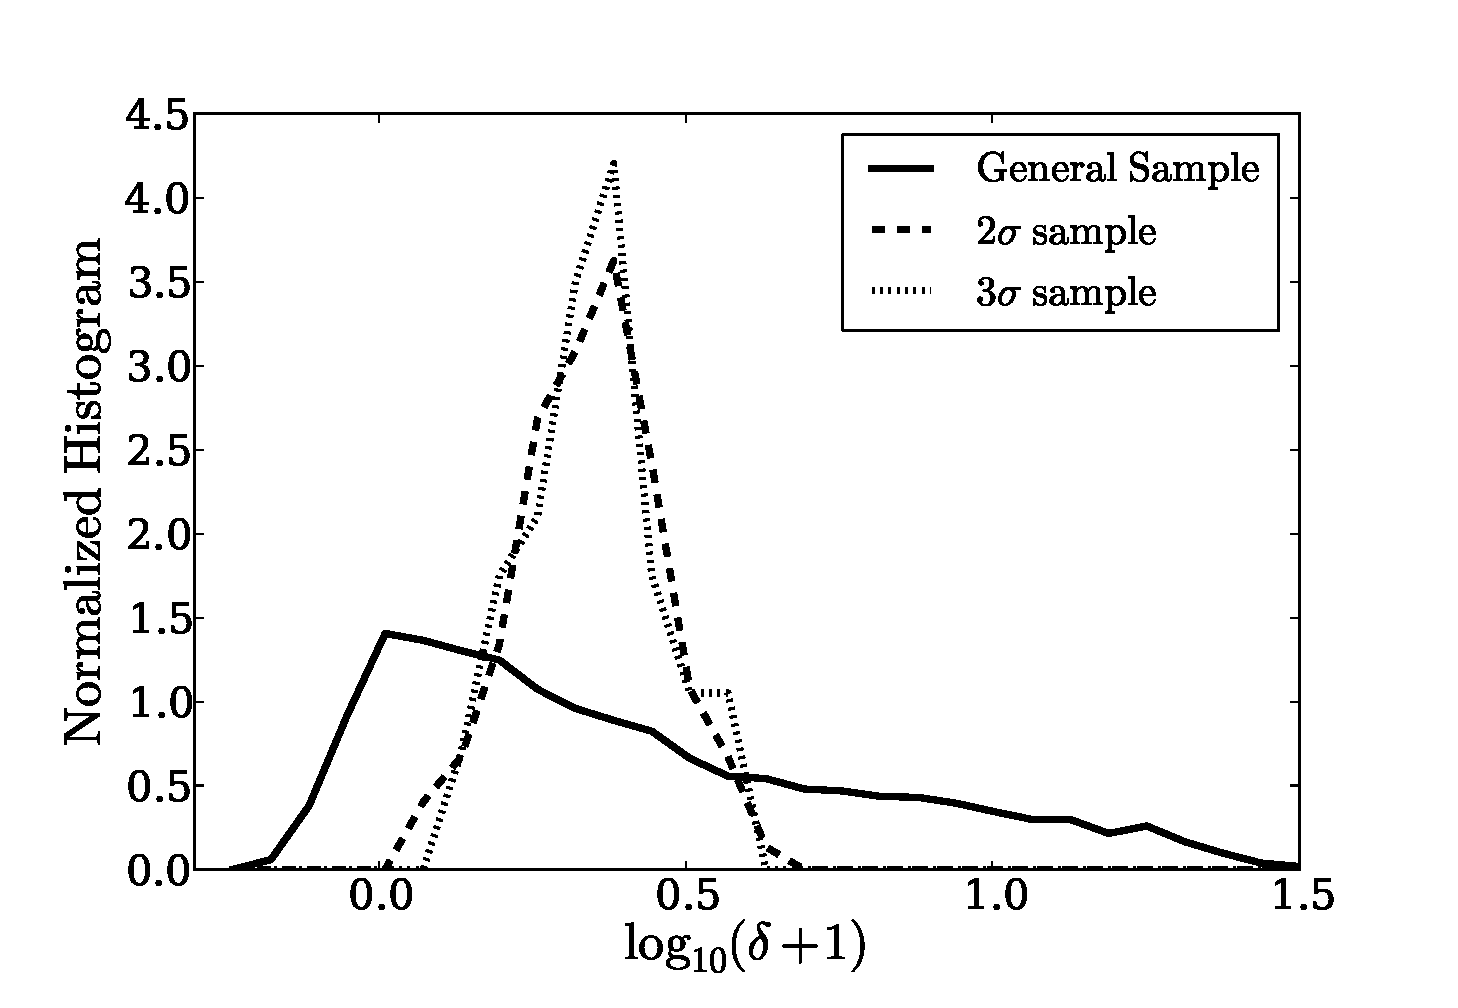
\includegraphics[width=0.45\textwidth]{density_histogram.eps}
\end{center}
\caption{Overdensity distribution for the pairs in the three samples.
    \label{fig:density}}  
\end{figure}


\begin{figure}
\begin{center}
  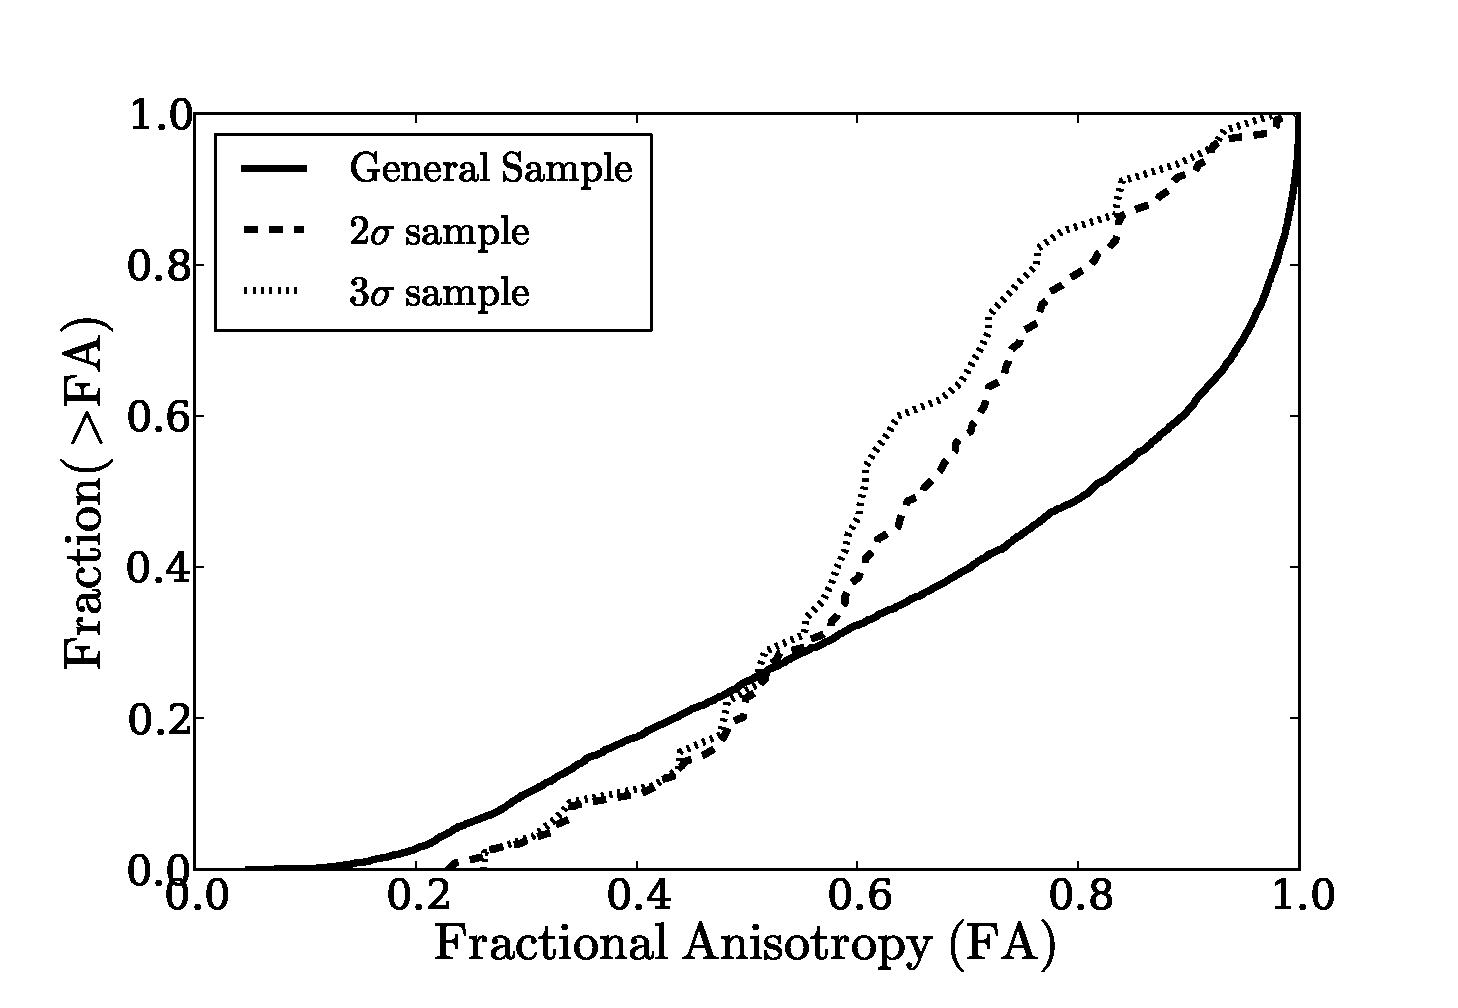
\includegraphics[width=0.45\textwidth]{FA_histogram.eps}
\end{center}
\caption{Integrated Fractional Anisotropy distribution for the pairs in the three samples.
    \label{fig:FA}}  
\end{figure}

\begin{figure}
\begin{center}
  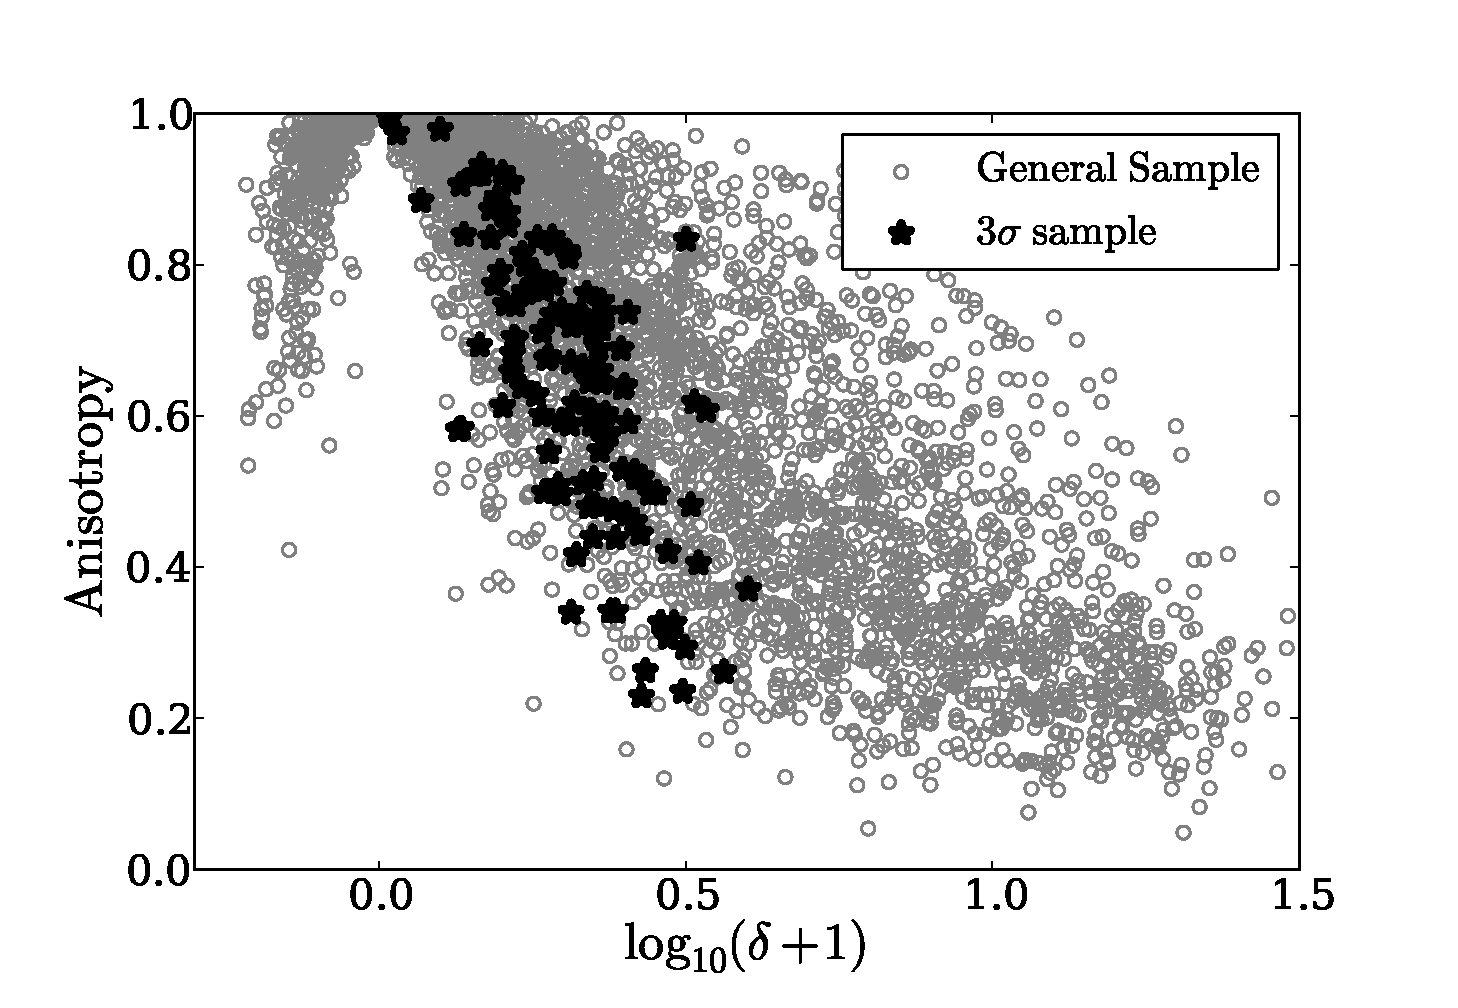
\includegraphics[width=0.45\textwidth]{FA_delta_scatter.eps}
\end{center}
\caption{Density and Fractional Anisotropy distribution for the pairs in the general and $3\sigma$ samples.
    \label{fig:FA}}  
\end{figure}

\section{Discussion}
\label{sec:discussion}

\section{Conclusions}
\label{sec:conclusions}


\section*{Acknowledgements}

\bibliographystyle{apj}
\bibliography{references} 


\end{document}


